\documentclass{article}
\usepackage{amsmath, amsthm, amssymb, amsfonts, bm}
\usepackage{graphicx}
\usepackage[T1]{fontenc}
\usepackage[utf8]{inputenc}
\usepackage[a4paper]{geometry}
\usepackage{fancyhdr}
\usepackage[algo2e]{algorithm2e}
\fontfamily{cmr}

\title{DD2424 - Assignment 1}
\author{Oskar Stigland \\ stigland@kth.se}

\pagestyle{fancy}
\fancyhf{}
\rhead{stigland@kth.se}
\lhead{DD2424 - Deep Learning in Data Science}
\rfoot{Page \thepage}

\begin{document}
%\maketitle

	\begin{titlepage}
		\begin{center} 
			
			\rule{\linewidth}{0.5mm}\\[0.5 cm]
			{ \huge \bfseries DD2424 - Assignment 1}\\[0.3 cm] % Title of your document
			\rule{\linewidth}{0.5mm}\\[1 cm]
					
			\small\vfill
			\begin{center}
			\centering
			{\large \bfseries \textsc{Summary}}\\
			\vspace{1cm}
			\begin{minipage}{10cm}
				
				I have written code for and completed all of the problems in the assignment. However, I believe there is some bug in the training which I cannot seem to resolve. The gradients have been checked and verified numerically, but for the first three sets of suggested parameter settings, my cost and loss is somewhat higher compared to the plot in the assignment description. At the same time, my obtained accuracy is lower. Looking at the weights, there are clear differences only when $\lambda = 1.0$. Other than this, I have implemented all of the features suggested in assignment description, including epoch-wise shuffling of the training data and both of the bonus problems.\\\\
%
	I have completed the code for the assignment in \texttt{python}. I have implemented the classificer as a class. For the hand-in, all of the code has been put toghether in a main file with all the functions and the class declared at the top. For the hand-in, I have also commented out the numerical gradient checking and the saving of generated figures. 
			\end{minipage}
			\end{center}
			\large\vfill
						

		\end{center}	
		
		\begin{minipage}{0.4\textwidth}
			\begin{flushleft} \large
				%\emph{Student:}\\
				Oskar \textsc{Stigland}\\
				DD2424\\
				Spring 2023
			\end{flushleft}
		\end{minipage}	

	\end{titlepage}

\newpage
\section*{Training the classifier}
\vspace{0.5cm}
\subsection*{Checking the gradients}
	I have checked the correctness of the analytically obtained gradients by comparing them to numerically computed gradients. For the latter, I have perturbed the full set of model parameters using a perturbation of $\epsilon = 10^{-5}$ and calculating the cost for a small subset of the training data. The maximum absolute errors for the weights and bias vectors are 

	\begin{align*}
		&\max_{\bm{w}}\, \big\vert\big\vert \nabla_{\bm{W}} J^{\text{analytical}} - \nabla_{\bm{W}} J^{\text{num}} \big\vert\big\vert < 10^{-9} \\
		&\max_{\bm{b}}\, \big\vert\big\vert \nabla_{\bm{b}} J^{\text{analytical}} - \nabla_{\bm{b}} J^{\text{num}} \big\vert\big\vert < 10^{-10}
	\end{align*}

\subsection*{Results}
	I initially tested the with the same parameter settings as the reported initial test in the assignment, i.e. \texttt{batchN} $=100$, \texttt{epochsN} $=40$, $\eta = 0.001$, and $\lambda = 0$. The results are shown in the figure below. Since $\lambda=0$, I have only included the loss for this particular example, which is shown together with the accuracy and the weights. As mentioned in the summary, the loss is surprisingly high. The accuracy obtained after $40$ epochs was $28.62$\%. There is also no discernable difference in the plotted weights. 
	\begin{figure}[h!]
		\centering
		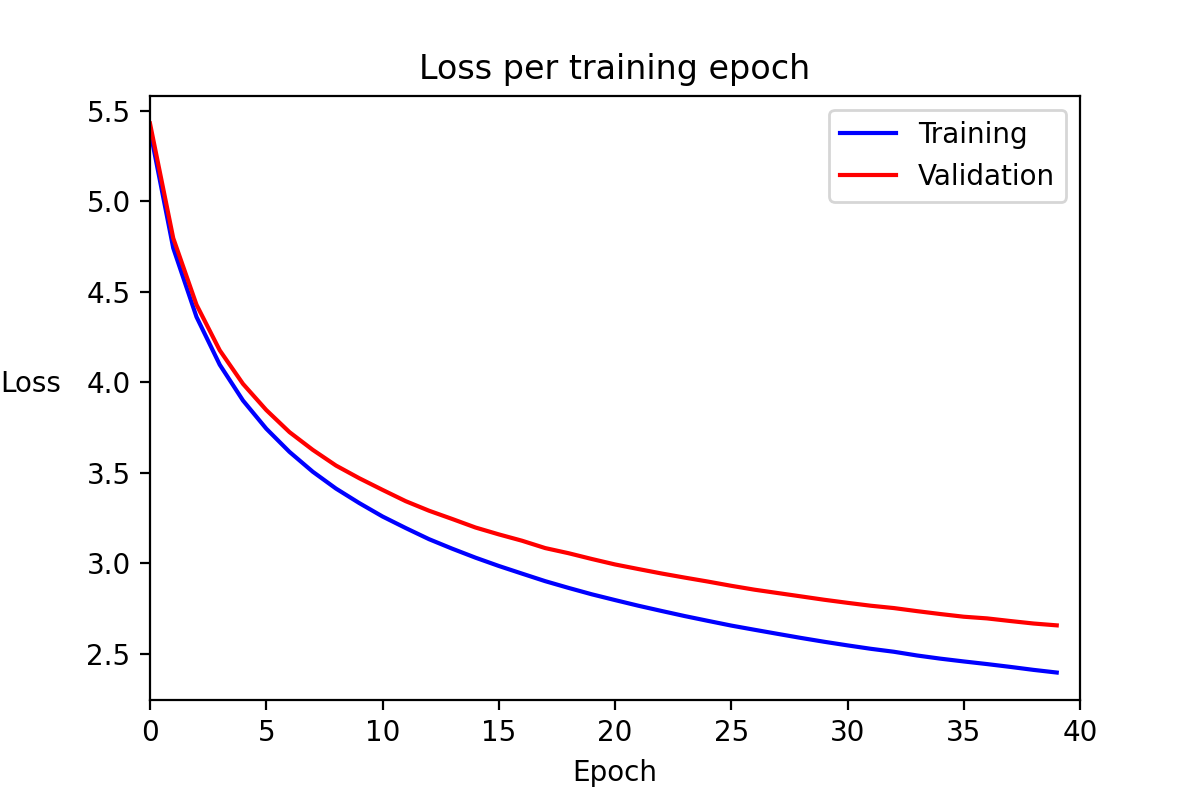
\includegraphics[width=7cm]{../plots/loss_v2.png}
		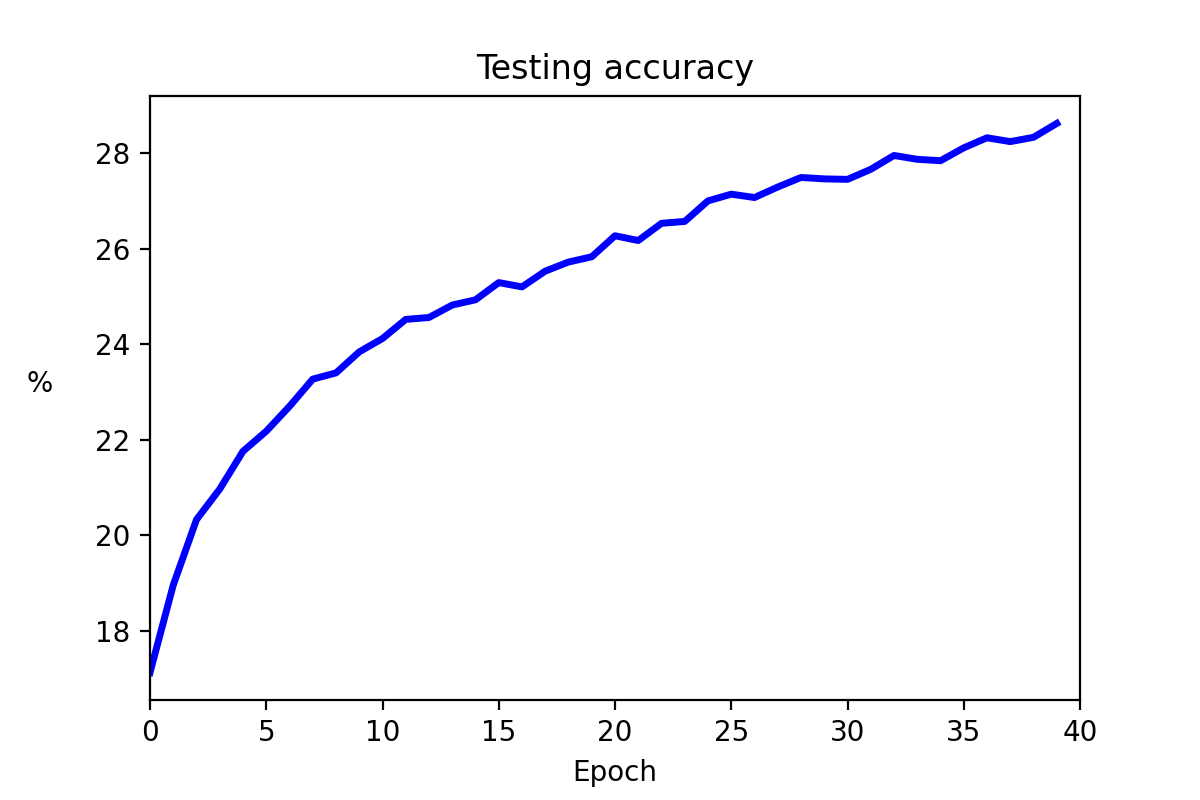
\includegraphics[width=7cm]{../plots/acc_v2.png}
		\caption{Loss and accuracy for initial set of parameters}
		\vspace{0.2cm}
		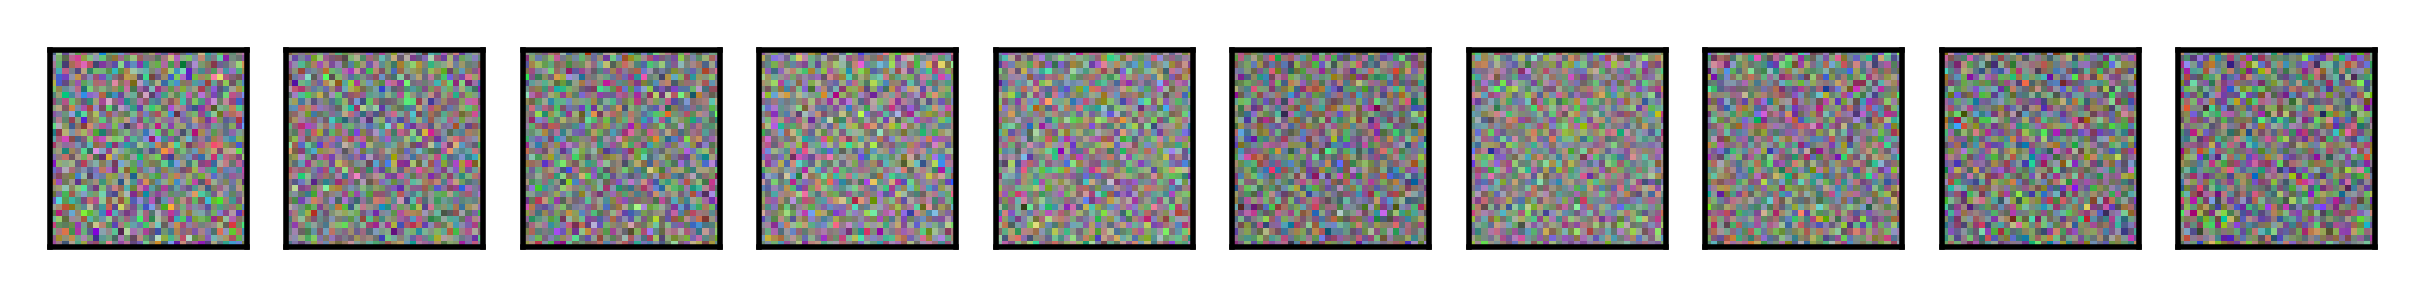
\includegraphics[width=12cm]{../plots/weights_v2.png}
		\caption{Class-specific weights for initial set of parameters}
		%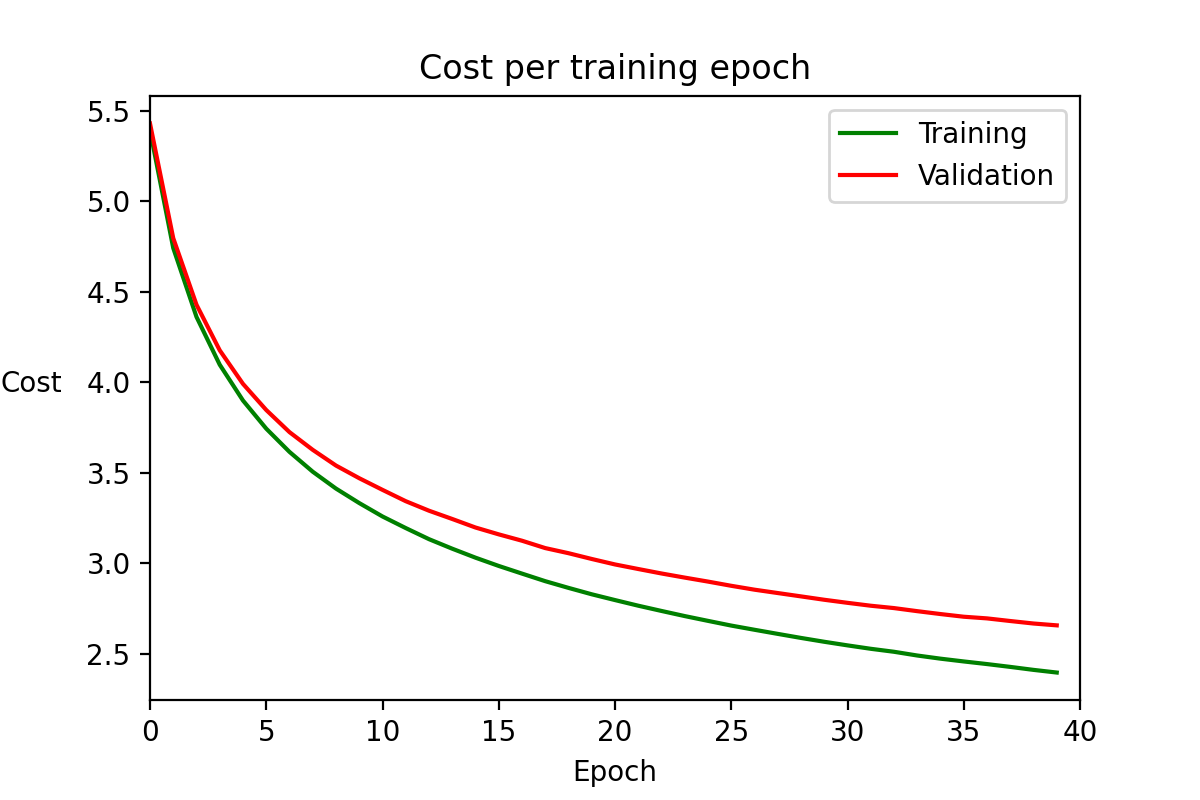
\includegraphics[width=7cm]{../plots/cost_v2.png}	
	\end{figure}\\
	As mentioned in the summary, there is likely some error. However, I have not been able to identify it. The gradients have been checked numerically. The results look a lot better and more convincing for the last set of parameters, i.e. where $\eta=0.001$ and $\lambda=1.0$. The training converges quickly and the training accuracy reaches $37.68$\% after $40$ epochs. Plotting the weights also show that the classes are somewhat discernable. The results are plotted below in the same fashion as for the initial parameter settings.

	\begin{figure}[h!]
		\centering
		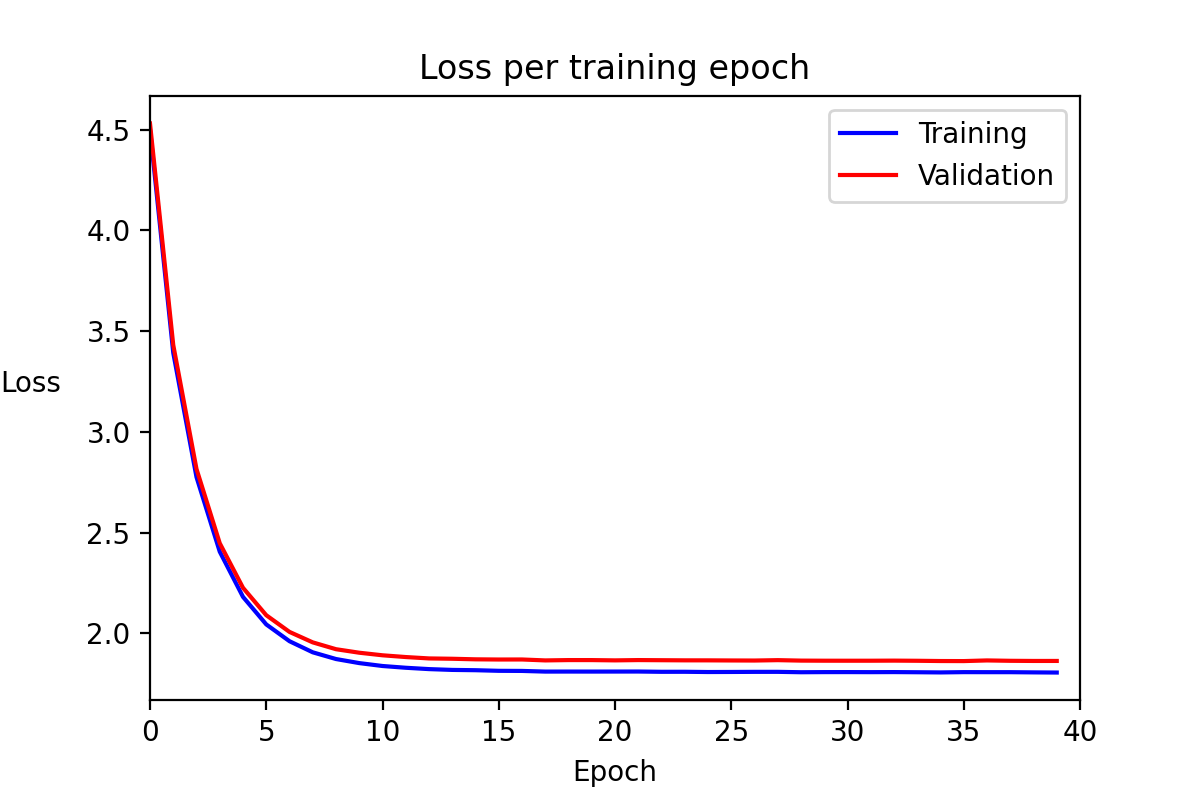
\includegraphics[width=7cm]{../plots/loss_v4.png}
		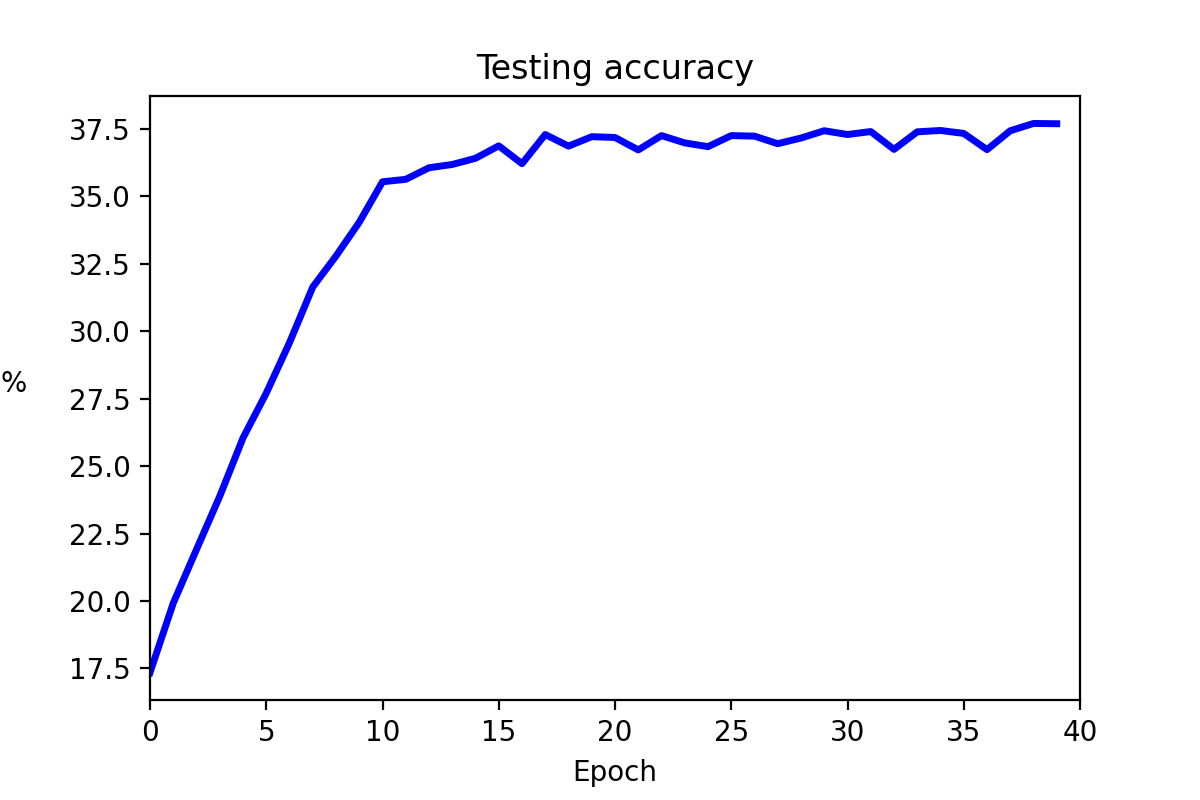
\includegraphics[width=7cm]{../plots/acc_v4.png}
		\caption{Loss and accuracy for $\eta=0.001$, $\lambda=1.0$}
		\vspace{0.2cm}
		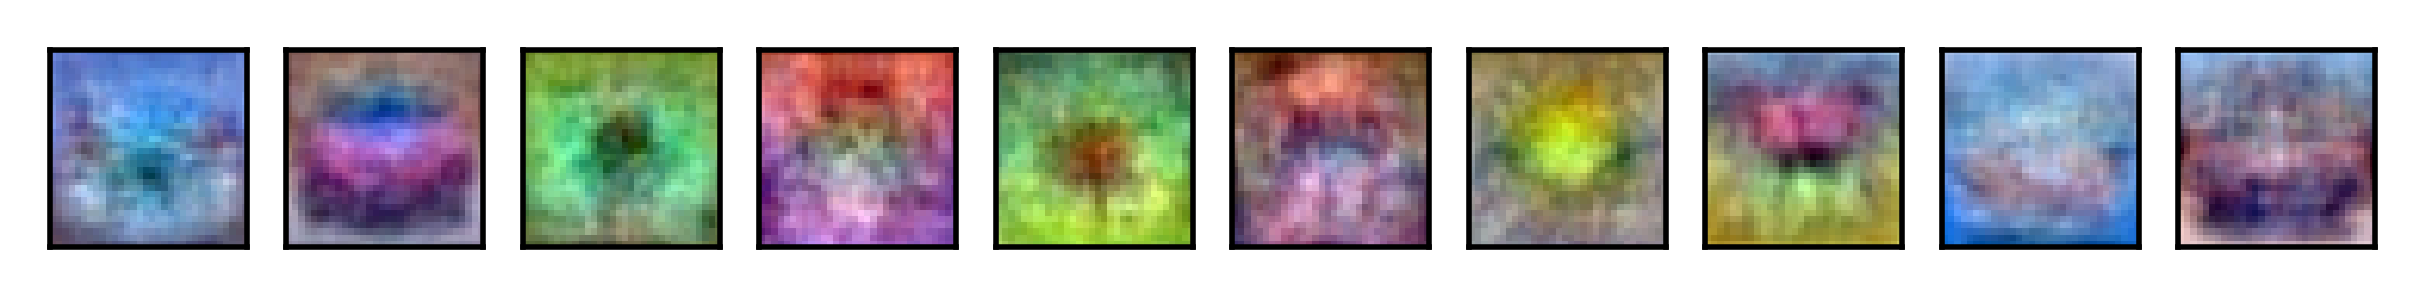
\includegraphics[width=12cm]{../plots/weights_v4.png}
		\caption{Class-specific weights for $\eta=0.001$, $\lambda=1.0$}
		%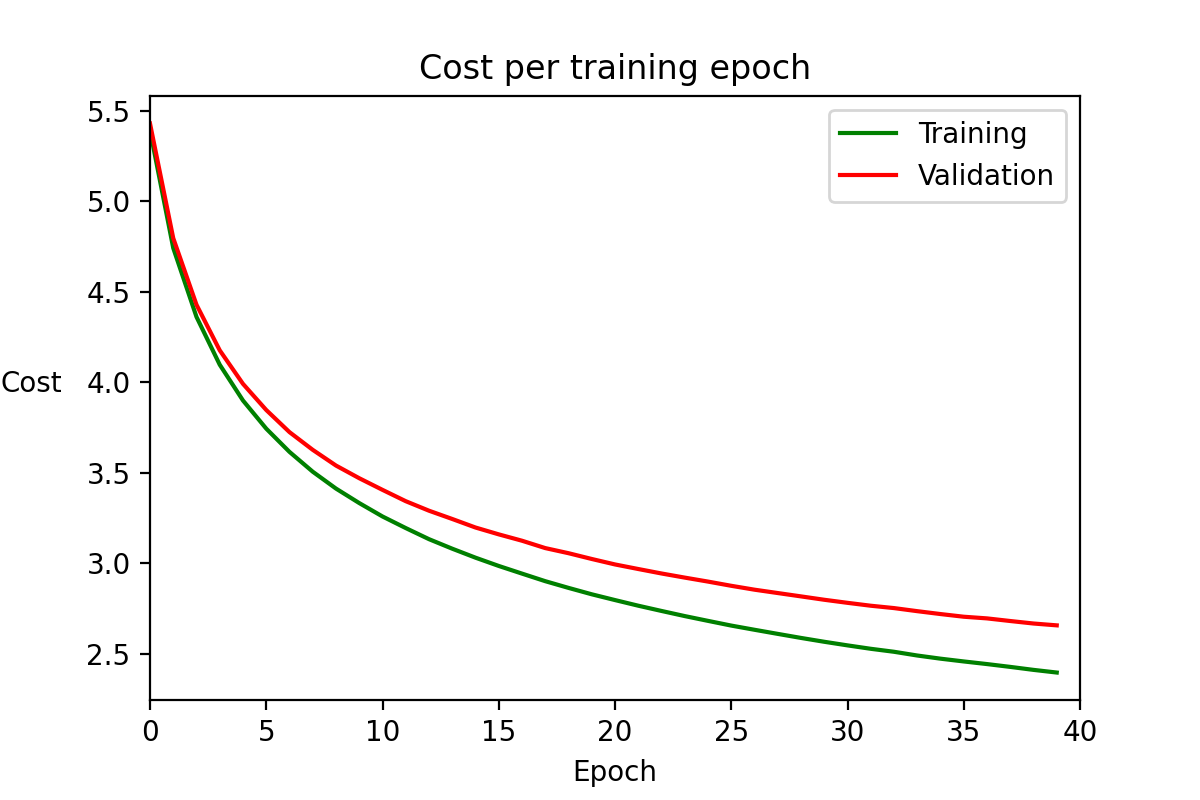
\includegraphics[width=7cm]{../plots/cost_v2.png}	
	\end{figure}

\subsection*{Results summary}
	I have trained the classifier for all four suggested sets of parameters. The results are summarized in the table below. Again, it becomes obvious that there is something not entirely correct in the training process. The accuracy for the first two parameter sets are almost identical, even the training is much more volatile in the former case. This is displayed in the set of plots on the last page. However, the performance clearly increases as we tune up the regularization parameter. For my implementation and the suggested parameter settings, I reached the best results with $\lambda = 1.0$. Although, these results should be taken with a grain of salt due to the suspected error. When I attempt to train for a longer period and a smaller batch size, e.g. \texttt{batchN} $=50$ and \texttt{epochsN} $=100$, with $\eta=0.001$ and $\lambda=0.0$, the model achieves an accuracy of $33.58$\%. The corresponding maximum accuracy when using $\eta=0.001$ and $\lambda=0.1$ is $39.74$\%. \\\\
%
In short, the turning up the regularization parameter clearly helps a lot in this particular case. The performance on the testing data gets significantly better with $\lambda > 0$. However, there are also other aspects of the training procedure which are clearly important to take into account, such as the learning rate, the batch size and the number of epochs. That is, performance does not increase in proportion to $\lambda$, since a lower $\lambda$ combined with e.g. a lower batch size actually achieves an even better result. It is also important to consider the learning rate, for which we clearly need a lower value in order to achieve a good result.

	\begin{center}
	\begin{tabular}{|l|l|l|l|c|}
		\hline
		\texttt{batchN} & \texttt{epochsN} & $\eta$ & $\lambda$ & \text{Accuracy}, \% \\ \hline
		100 & 40 & 0.1 & 0.0 & 28.37 \\
		100 & 40 & 0.001 & 0.0 & 28.62\\
		100 & 40 & 0.001 & 0.1 &  33.37\\
		100 & 40 & 0.001 & 1.0 & 37.68\\ 
		50 & 100 & 0.001 & 0.1 & 39.74\\
		50 & 100 & 0.001 & 0.5	 & 38.75\\
		50 & 100 & 0.001 & 1.0 & 37.93\\\hline
	\end{tabular}
	\end{center}

\newpage

	\begin{figure}[h!]
		\centering
		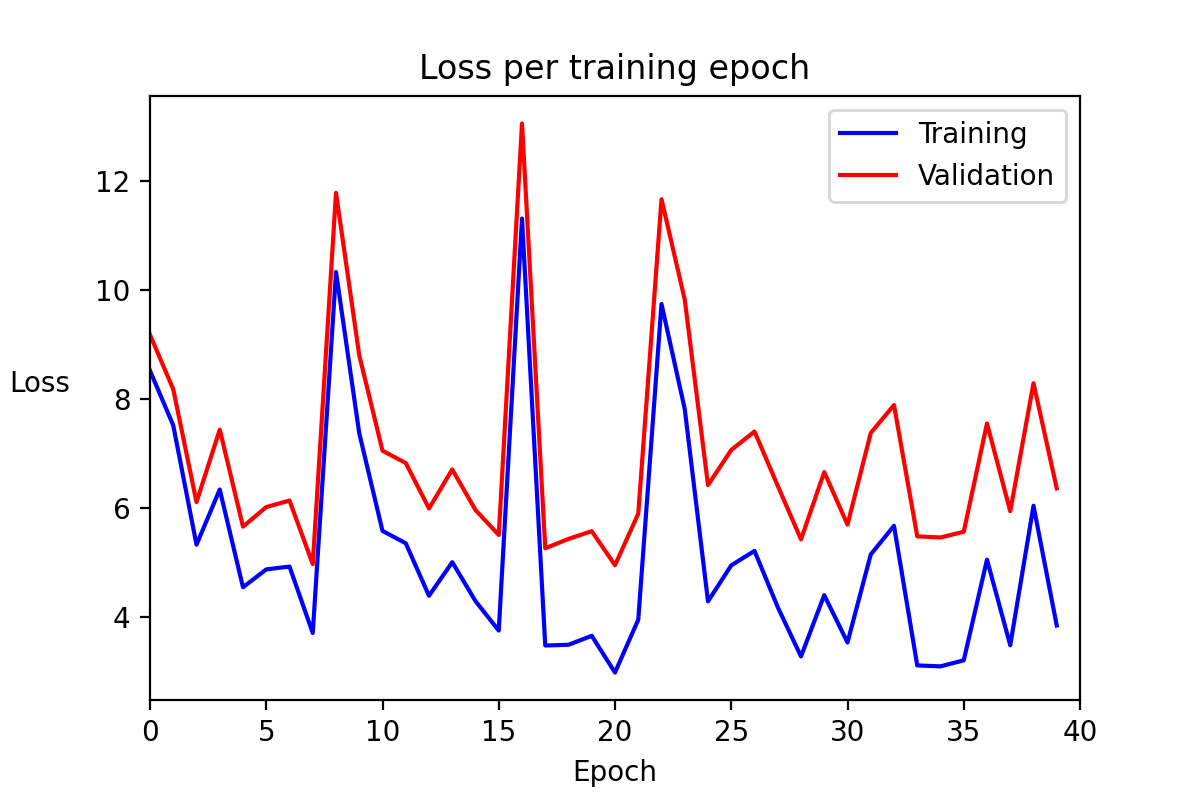
\includegraphics[width=6cm]{../plots/loss_v1.png}
		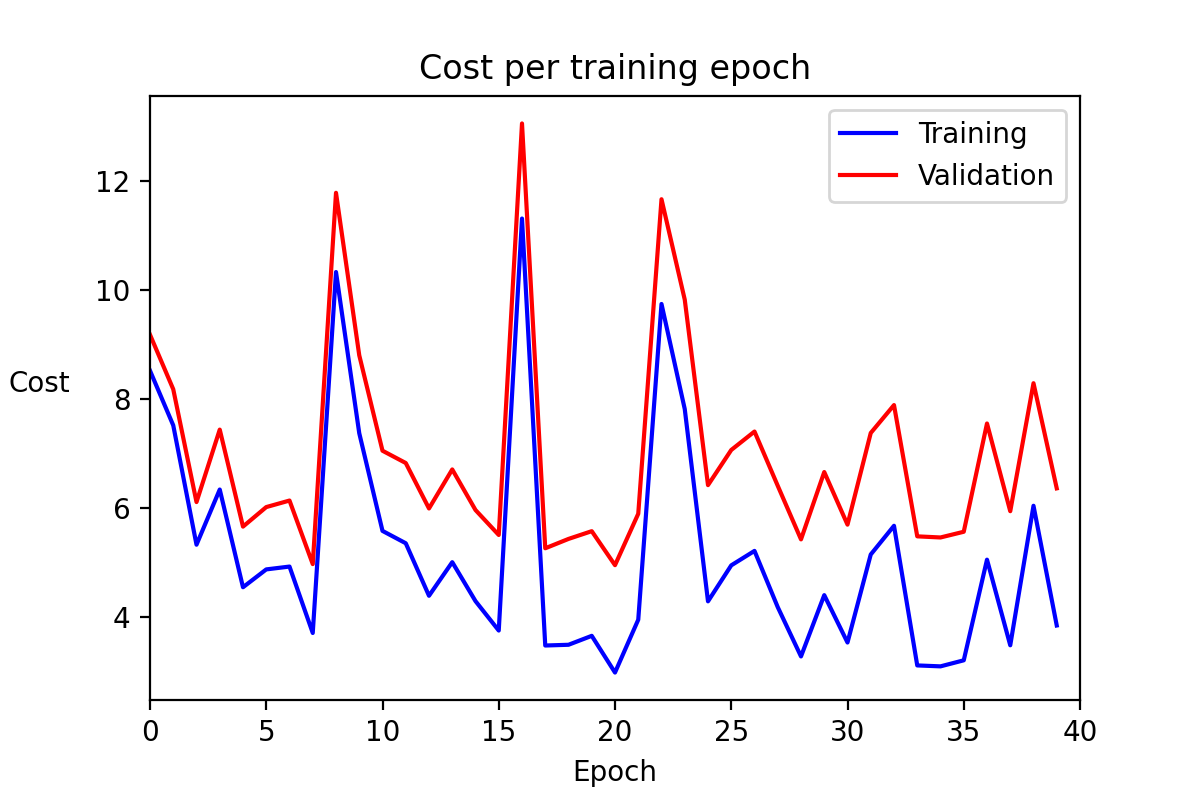
\includegraphics[width=6cm]{../plots/cost_v1.png}
		\caption{Loss and accuracy for $\eta=0.1$, $\lambda=0.0$}
		\vspace{0.2cm}
		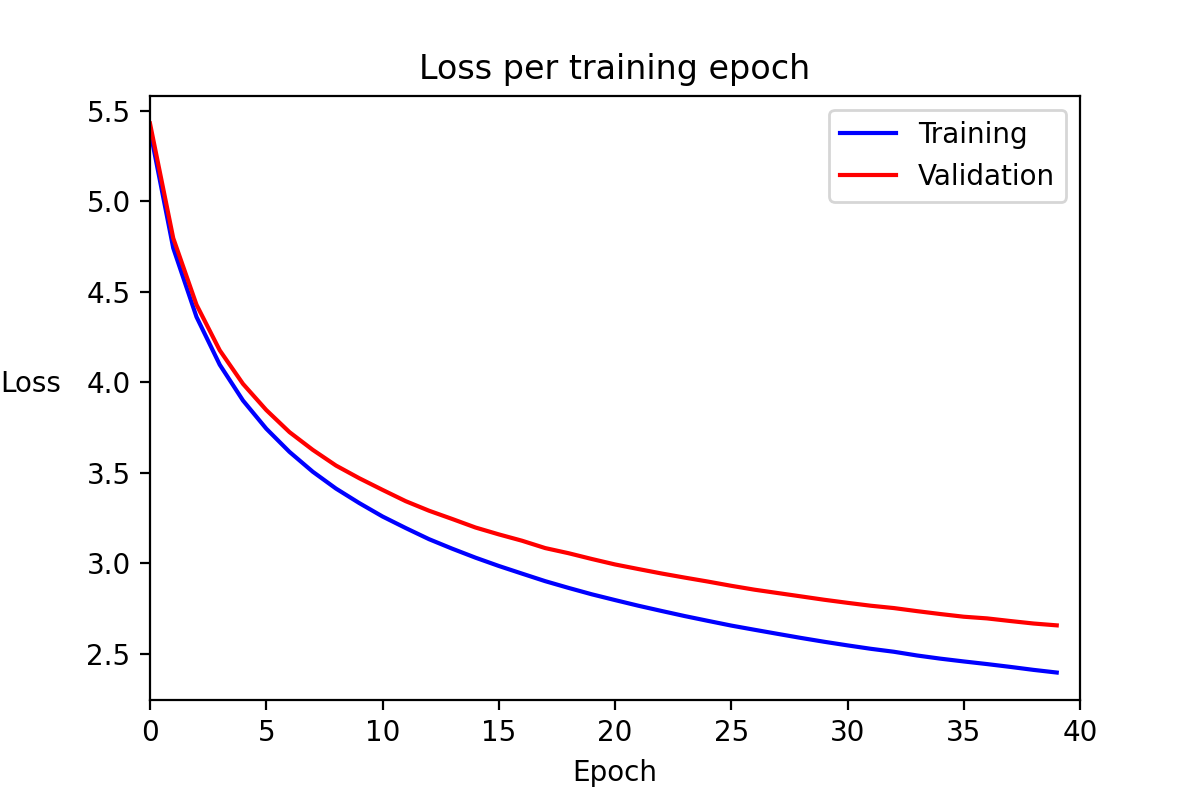
\includegraphics[width=6cm]{../plots/loss_v2.png}
		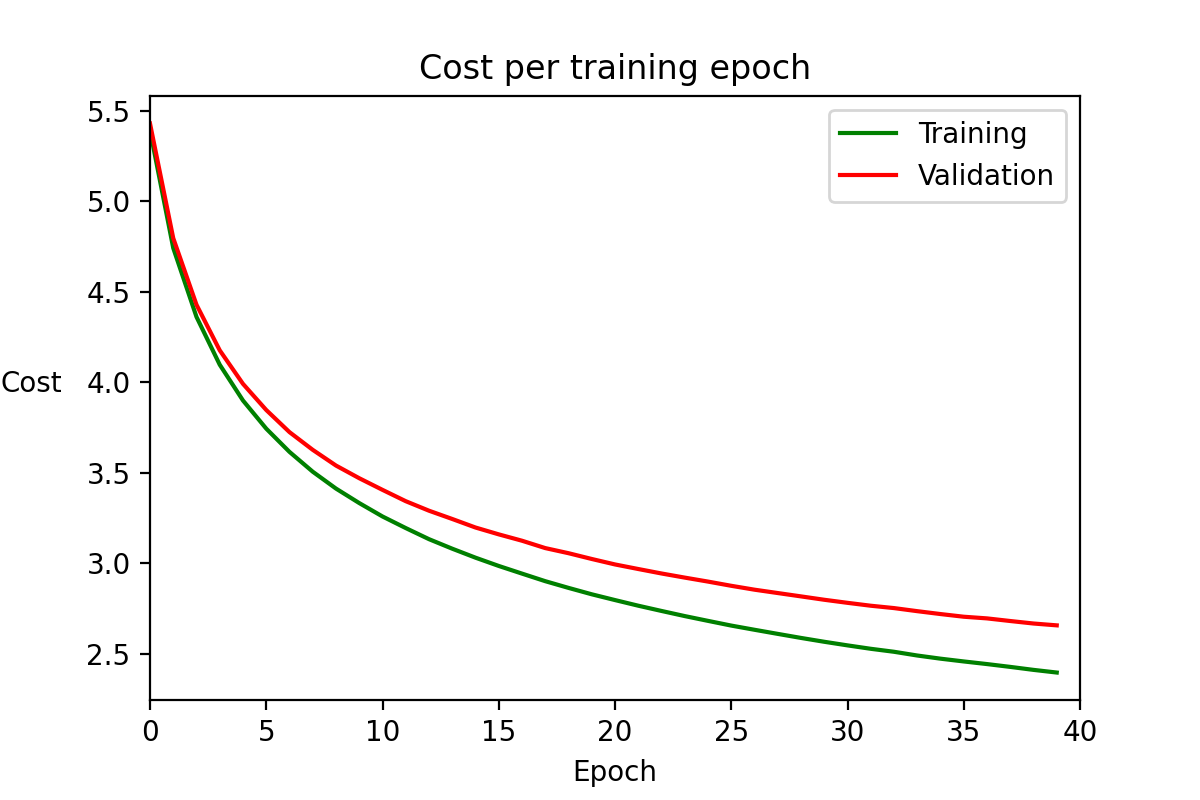
\includegraphics[width=6cm]{../plots/cost_v2.png}
		\caption{Loss and accuracy for $\eta=0.001$, $\lambda=0.0$}
		\vspace{0.2cm}
		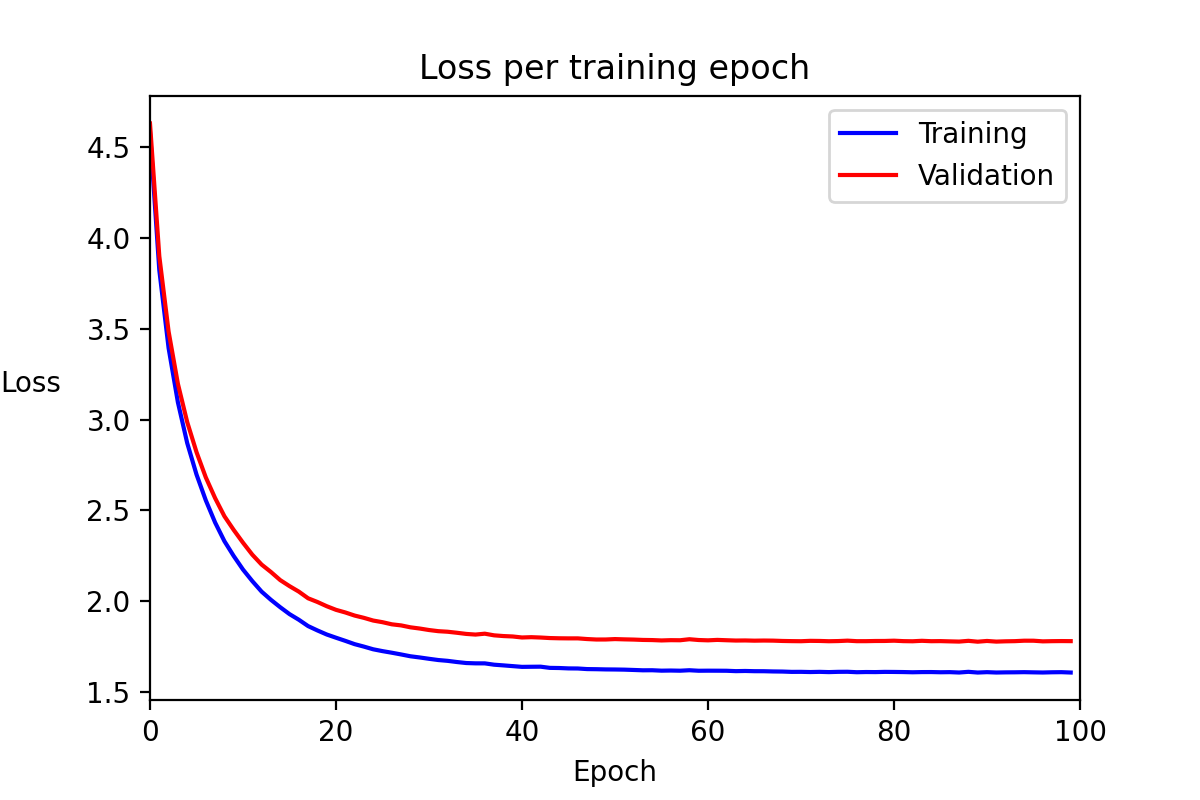
\includegraphics[width=6cm]{../plots/loss_v3.png}
		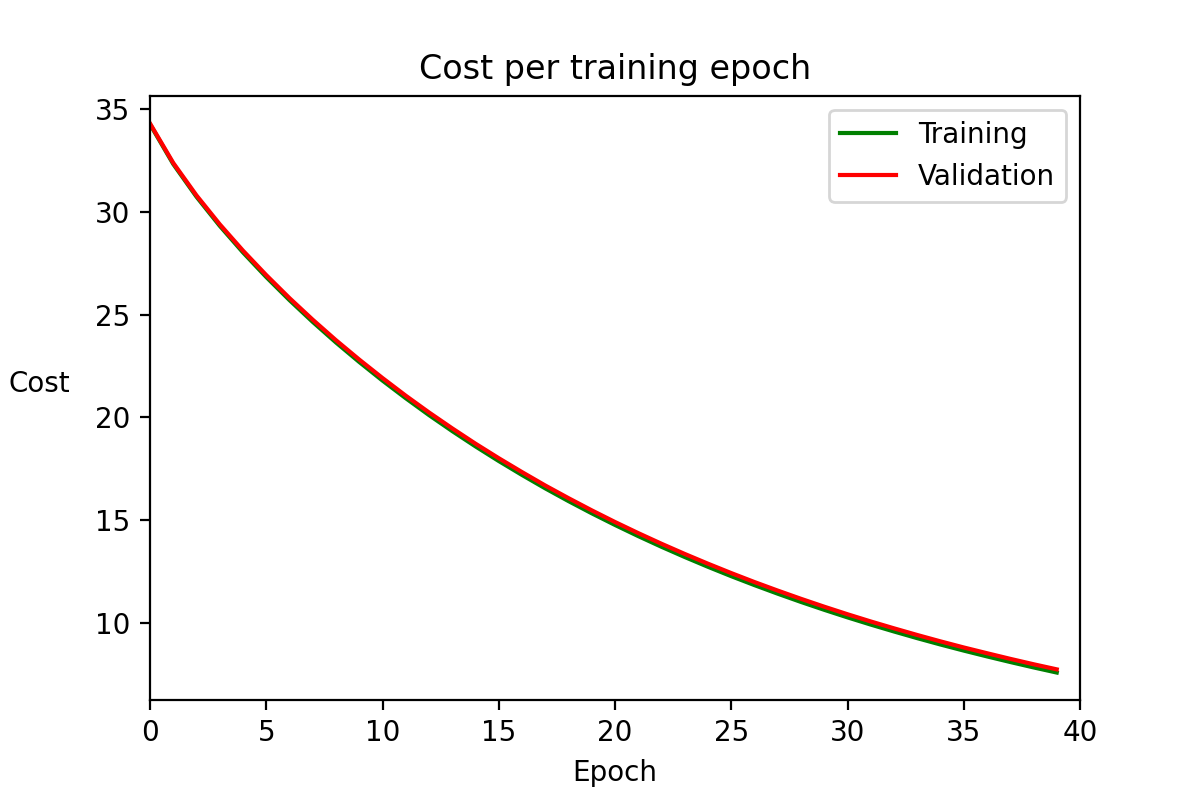
\includegraphics[width=6cm]{../plots/cost_v3.png}
		\caption{Loss and accuracy for $\eta=0.001$, $\lambda=0.1$}
		\vspace{0.2cm}
		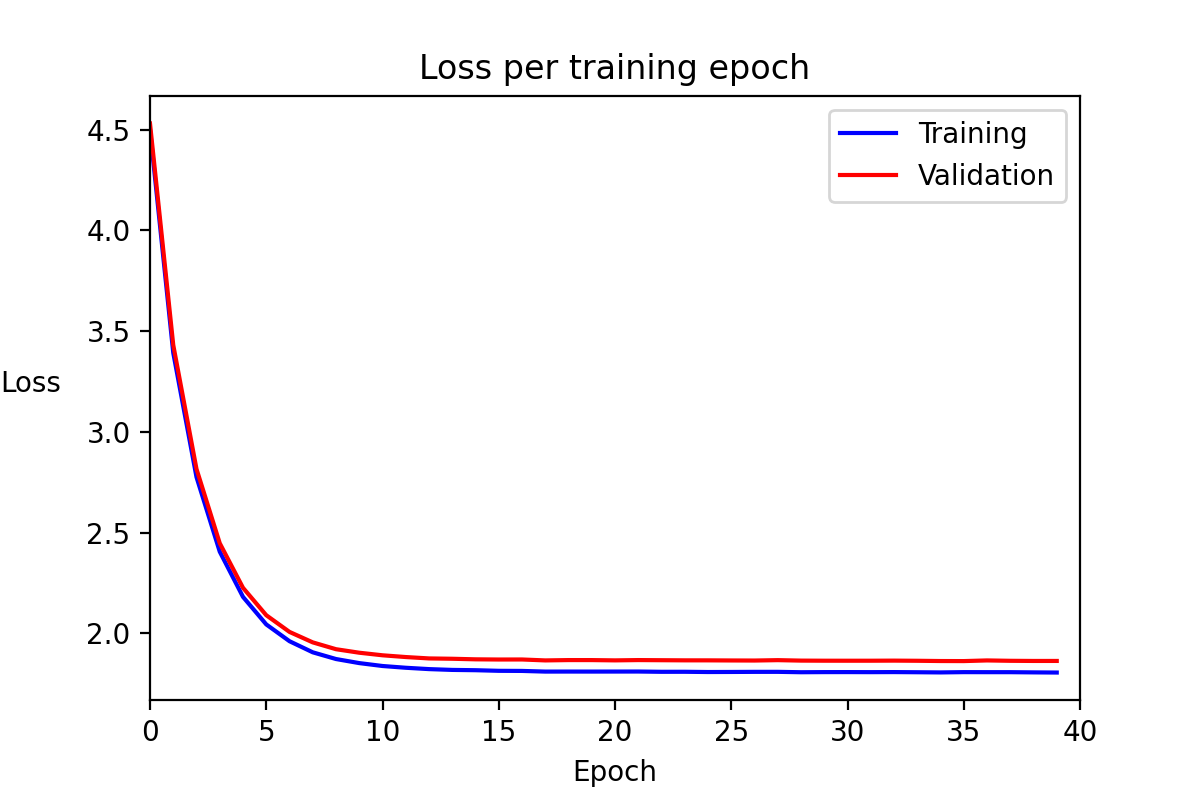
\includegraphics[width=6cm]{../plots/loss_v4.png}
		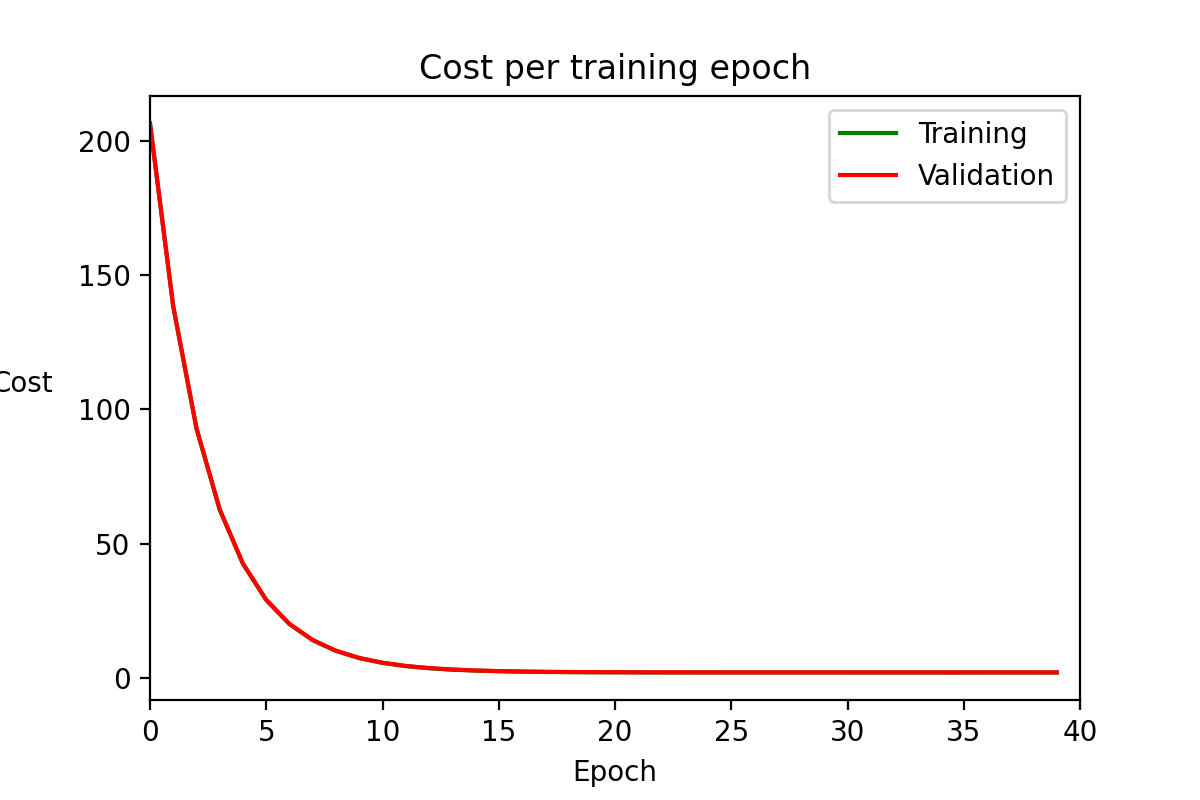
\includegraphics[width=6cm]{../plots/cost_v4.png}
		\caption{Loss and accuracy for $\eta=0.001$, $\lambda=1.0$}
		\vspace{0.2cm}
	\end{figure}
	

\end{document}